\section{Evaluation der Implementation mit echten Logdateien}
In diesem Abschnitt verwendeten wir unsere Implementierung für die Analyse von \gls{ssh}-Logdateien der Hochschule. Für die Extrahierung der Dateien bekommt unseren Promtail-Instanz folgende Konfiguration:

{\setstretch{1.0}
\begin{Verbatim}[frame=single,fontsize=\small]
scrape_configs:
- job_name: sshlogs
  decompression:
    enabled: true
    initial_sleep: 15s
    format: gz
  static_configs:
  - targets:
      - localhost
    labels:
      job: sshlogs
      instance: Opfersystem1
      __path__: /var/log/**.gz
\end{Verbatim}
}

Promtail sucht automatisch und nach vordefinierten Zeitabstand nach Logdateien, die in der Konfigurationsdatei eintregagen wurden. Unten befindet sich die Erklärung jedes Elements dieser Einstellung:

\begin{table}[H]
    \setstretch{1}
    \begin{tabularx}{\textwidth}{|m{5.5cm}|X|}
    \hline
    \multicolumn{1}{|c|}{\textbf{Konfigurationsfeld}} & \multicolumn{1}{|c|}{\textbf{Beschreibung}} \\
    \hline
    scrape\_configs & Bezieht sich auf die Funktionalität von Promtail automatisch nach Logdatein zu suchen. \\
    \hline
    decompression \newline
    \hphantom{12}enabled: true \newline
    \hphantom{12}initial\_sleep: 10s \newline
    \hphantom{12}format: gz & Promtail kann die einige Komprimierungsformate verarbeiten, unter denen .gz, was wir in unserer Arbeit benutzen. Der field \quotes{initial\_sleep} beschreibt die Intervallzeit, bevor die Dekomprimierung anfängt. Dieser Felt kann nützlich sein, wenn komprimierte Datei vorhanden sind aber deren Komprimierungsverfahren noch nicht abschlossen ist. Der Feld Format deutet auf die Komprimierungsformate hin \citep{Grafana_Promtail}.  \\
    \hline
    \end{tabularx}
\end{table}

\begin{table}[H]
  \setstretch{1}
  \begin{tabularx}{\textwidth}{|m{5.5cm}|X|}
  \hline
  \multicolumn{1}{|c|}{\textbf{Konfigurationsfeld}} & \multicolumn{1}{|c|}{\textbf{Beschreibung}} \\
  \hline
  static\_configs: \newline
  \hphantom{1}- targets: \newline
  \hphantom{123}- localhost \newline
  \hphantom{1}labels: \newline
  \hphantom{123}job: sshlogs \newline
  \hphantom{123}\_\_path\_\_: /var/log/**.gz & \quotes{targets} bezieht sich auf die Kommunikation mit dem Loki-Instanz. \quotes{labels} zeigt, mit welcher Identifizierung den Inhalt dieser Datei im Loki aufgerufen werden kann. \quotes{\_\_path\_\_} gibt an, wo sich die Datei im System befinden\\
  \hline
  %sample\_rate: 0.1 & , which means that Promtail will sample 10% of the series during scraping. \\
  %\hline
  \end{tabularx}
  \caption[Schnipsel der verwendeten Konfigurationsdatei von Promtail]
  {Schnipsel der verwendeten Konfigurationsdatei von Promtail}
\end{table}

\quotes{Labels} spielen eine wesentliche Rolle in der Performance bei Loki, da dieses Tool mit weniger Indexierung als anderes Tool, wie Elastic Stack, arbeitet. \cite{Grafana_labels} empfiehl so wenig \quotes{labels} wie möglich zu verwenden, die Extrahierung von Inhalt sollte stattdessen mithilfe der \gls{abfragesprache} stattfinden, um eine Eskalation bei der Speicherung zu vermeiden. Die Abbildung \ref{fig:Eskalation_Labels} zeigt den Effekt von mehreren Labels auf die Anwendung:

\begin{figure}[H]
  \centering
  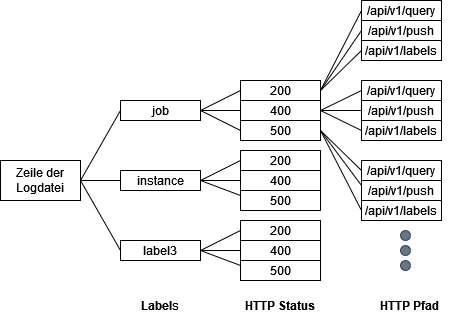
\includegraphics[width=0.7\textwidth]{assets/labelstream.png}
  \caption[Eskalation bei der Indexierung]
  {Eskalation bei der Indexierung Labels laut \cite{Grafana_labels}}
  \label{fig:Eskalation_Labels}
  \centering
\end{figure}

Auf der Abbildung \ref{fig:Eskalation_Labels} haben wir vier Ebenen. Die erste ist die Zeile der Logdatei, die zweite ist die von den Benutzer definierten \quotes{labels} und die dritte und vierte beziehen sich auf die Antwort und auf die verwendeten \gls{http}-Anfrage, um nach Inhalt abzufragen, hinzuzufügen und zu indexieren. Aus einer Zeile der Logdatei werden drei \quotes{labels} (3x), diese haben wiederum drei potentielen Status (3x3x) aus drei notwendigen \gls{http}-Pfad (3x3x3). Aus einer Zeilen hätten wir schließlich 27 Streams, um die Zeile zu lesen, zu indexieren und zu speichern. Das kann laut \cite{Grafana_labels} zu mangelnden Leistungsfähigkeit führen.


\textcolor{red}{\textbf{Noch etwas zu unserem Ergebnis hinzufügen}}
\textcolor{red}{\textbf{Status: 500. Message: too many outstanding requests}}



\newpage
\newgeometry{right=30mm, left=30mm} 
\thispagestyle{lscape}
\begin{landscape}
   Die Ausgabe in Grafana nach dem Hinzufügen unserer Logdateien ist auf der Abbildung \ref{fig:Unserssh} dargestellt:
    \begin{figure}[H]
       % \centering
        \centerline{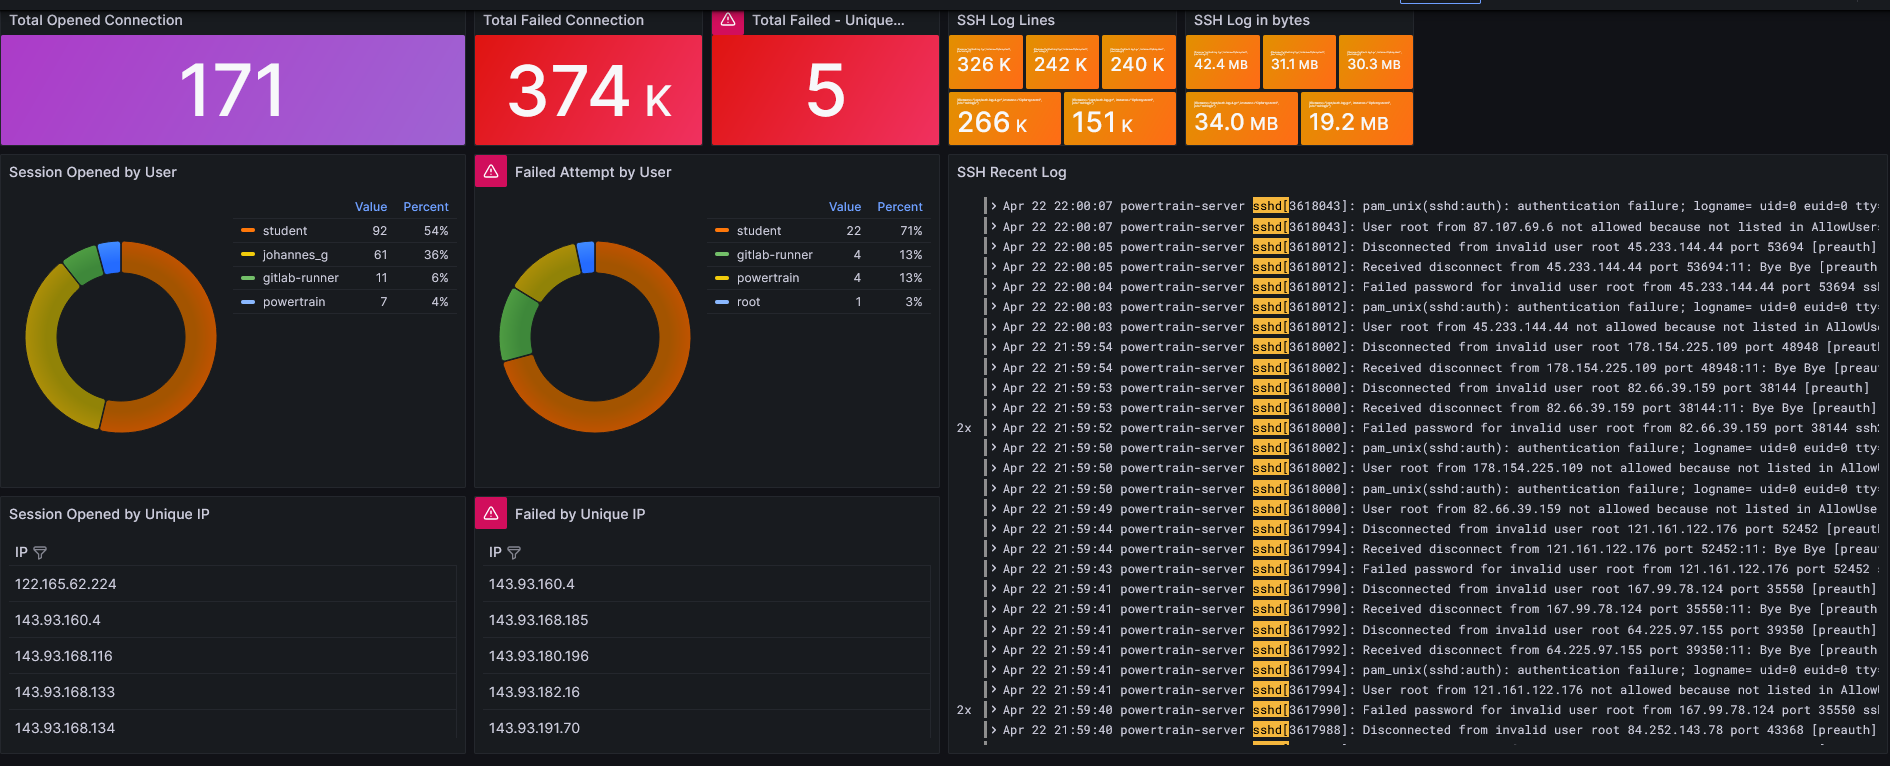
\includegraphics[width=1.8\textwidth]{assets/unserssh}}
        %\includegraphics[width=1.2\textwidth]{assets/5.4.2_1_Abb.jpeg}
        \caption[Ausgabe in Grafana von unseren \gls{ssh} Logdateien]
        {Ausgabe in Grafana von unseren \gls{ssh} Logdateien}
        \label{fig:Unserssh}
        \centering
    \end{figure} 
\end{landscape}
\restoregeometry


%  In the Promtail configuration file, the initial_sleep field is used to specify the initial delay before Promtail starts scraping logs from a given file.

%  When Promtail starts up, it needs to read the log files from the beginning to identify where it left off, and then begin tailing the logs from that point forward. If the log file is large or there are many log files to be read, this initial indexing process can take some time.
 
%  The initial_sleep field specifies the number of seconds that Promtail should wait before starting to read logs from a given file. This delay can be used to give the indexing process more time to complete before Promtail begins tailing the logs.
 
%  For example, if you have a large log file that takes several minutes to index, you might set the initial_sleep field to a few minutes to ensure that the indexing process is complete before Promtail starts scraping logs.
 
%  Note that the initial_sleep field is optional and defaults to 0 seconds if not specified.
